\documentclass[tikz,border=2pt]{standalone}
\usepackage{amsmath}
\usepackage{amssymb}
\usepackage{xcolor}
\usepackage{tikz}
\usetikzlibrary{arrows.meta,positioning,fit,backgrounds,calc,shapes.geometric}

% ---------- palette ----------
\definecolor{accentA}{HTML}{2E7D5B}
\definecolor{accentB}{HTML}{2F5BAA}
\definecolor{panelA}{HTML}{EAF2EA}
\definecolor{panelB}{HTML}{EAF0FA}
\definecolor{fillB}{HTML}{CBDCF3}
\definecolor{edge}{HTML}{6B7280}
\definecolor{ink}{HTML}{1F2937}
\definecolor{muted}{HTML}{9AA3AF}
\definecolor{haloA}{HTML}{DDEBDD}

\begin{document}
\sffamily
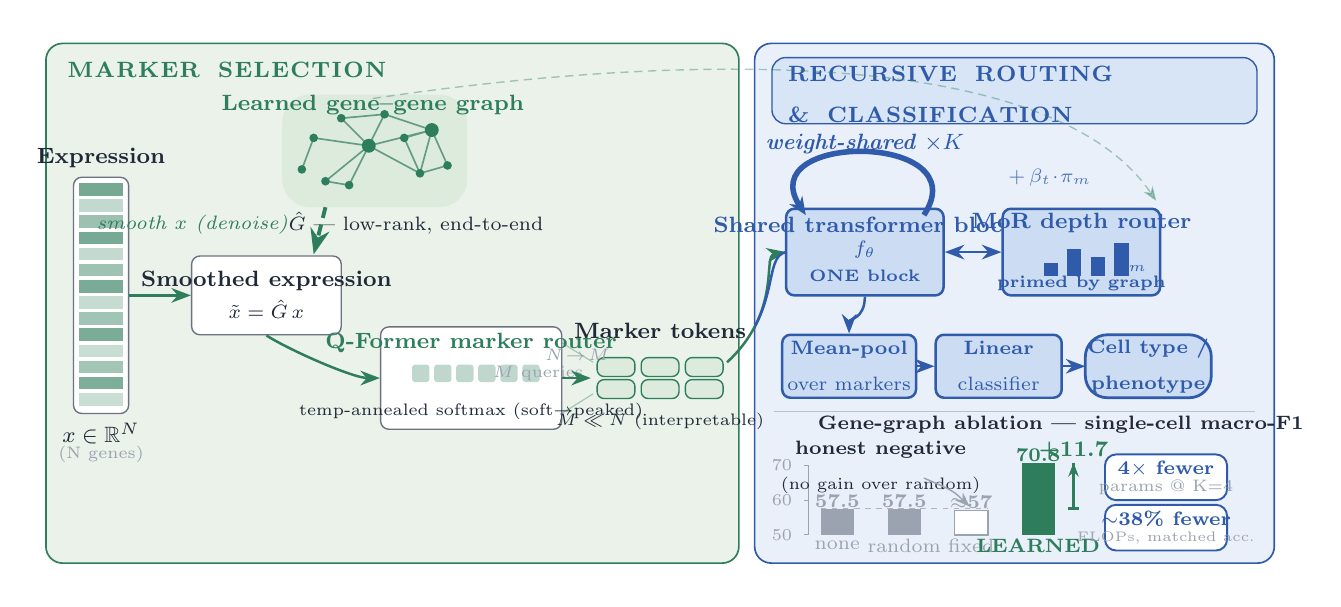
\begin{tikzpicture}[x=1cm,y=1cm,>=Stealth,
  stagebox/.style={draw=edge,line width=0.5pt,fill=white,rounded corners=3pt},
  stageboxB/.style={draw=accentB,line width=0.9pt,fill=fillB,rounded corners=3pt},
  flow/.style={draw,line width=0.9pt,->}]

% ==================================================================
% 0. CANVAS (invisible bounds 16 x 7)
% ==================================================================
\path (0,0) rectangle (16,7);

% ==================================================================
% 1. PANELS (behind everything)
% ==================================================================
\begin{scope}[on background layer]
  \draw[fill=panelA,draw=accentA,line width=0.6pt,rounded corners=6pt]
    (0.20,0.20) rectangle (9.00,6.80);
  \draw[fill=panelB,draw=accentB,line width=0.6pt,rounded corners=6pt]
    (9.20,0.20) rectangle (15.80,6.80);
\end{scope}

% panel A label (extreme top-left corner)
\node[anchor=north west,accentA] at (0.35,6.68)
  {\bfseries\footnotesize\scshape M\kern0.5pt A\kern0.5pt R\kern0.5pt K\kern0.5pt E\kern0.5pt R\ \ S\kern0.5pt E\kern0.5pt L\kern0.5pt E\kern0.5pt C\kern0.5pt T\kern0.5pt I\kern0.5pt O\kern0.5pt N};

% panel B header band (clear top-left header, blocks pushed below it)
\begin{scope}[on background layer]
  \draw[fill=fillB,draw=accentB,line width=0.5pt,rounded corners=5pt,fill opacity=0.55]
    (9.42,5.78) rectangle (15.58,6.62);
\end{scope}
\node[anchor=north west,accentB,align=left,inner sep=0pt] at (9.62,6.52)
  {\bfseries\footnotesize\scshape R\kern0.3pt E\kern0.3pt C\kern0.3pt U\kern0.3pt R\kern0.3pt S\kern0.3pt I\kern0.3pt V\kern0.3pt E\ \ R\kern0.3pt O\kern0.3pt U\kern0.3pt T\kern0.3pt I\kern0.3pt N\kern0.3pt G\\[0.10cm]
   \bfseries\footnotesize\scshape \&\ \ C\kern0.3pt L\kern0.3pt A\kern0.3pt S\kern0.3pt S\kern0.3pt I\kern0.3pt F\kern0.3pt I\kern0.3pt C\kern0.3pt A\kern0.3pt T\kern0.3pt I\kern0.3pt O\kern0.3pt N};

% panel B divider
\draw[muted,line width=0.4pt,opacity=0.6] (9.45,2.12) -- (15.55,2.12);

% ==================================================================
% 2. PANEL A NODES
% ==================================================================

% --- n_input : heat strip ---
\node[stagebox,minimum width=0.70cm,minimum height=3.00cm] (n_input)
  at (0.90,3.60) {};
\foreach \i in {0,...,13}{
  \pgfmathsetmacro{\yy}{2.20+\i*0.205}
  \pgfmathsetmacro{\op}{25+mod(\i*37,55)}
  \fill[accentA,opacity=\op/100] (0.62,\yy) rectangle (1.18,\yy+0.16);
}
\node[ink] at (0.90,5.35) {\bfseries\footnotesize Expression};
\node[ink] at (0.90,1.85) {\footnotesize $x \in \mathbb{R}^{N}$};
\node[muted] at (0.90,1.58) {\fontsize{6.5}{7.5}\selectfont (N genes)};

% --- n_graph HERO (pushed up + right, clear of the corner label) ---
\begin{scope}[on background layer]
  \fill[haloA,rounded corners=10pt] (3.20,4.72) rectangle (5.55,6.15);
\end{scope}
% graph nodes
\coordinate (g1) at (3.75,5.05);
\coordinate (g2) at (4.30,5.50);   % hub
\coordinate (g3) at (4.95,5.15);
\coordinate (g4) at (3.60,5.60);
\coordinate (g5) at (4.50,5.90);
\coordinate (g6) at (5.10,5.70);   % hub
\coordinate (g7) at (4.05,5.00);
\coordinate (g8) at (4.75,5.60);
\coordinate (g9) at (3.95,5.85);
\coordinate (g10) at (5.30,5.25);
\coordinate (g11) at (3.45,5.20);
\draw[accentA,line width=0.6pt,opacity=0.7]
  (g2)--(g1) (g2)--(g4) (g2)--(g7) (g2)--(g9) (g2)--(g5) (g2)--(g3)
  (g6)--(g3) (g6)--(g5) (g6)--(g8) (g6)--(g10) (g6)--(g2)
  (g5)--(g9) (g3)--(g10) (g4)--(g11) (g1)--(g7) (g8)--(g3);
\foreach \g in {g1,g3,g4,g5,g7,g8,g9,g10,g11}
  \fill[accentA] (\g) circle (0.055);
\fill[accentA] (g2) circle (0.088);
\fill[accentA] (g6) circle (0.088);
\node[accentA] at (4.35,6.02) {\bfseries\footnotesize Learned gene--gene graph};
% Ghat caption BELOW the cluster
\node[ink] at (4.90,4.52) {\fontsize{7}{8}\selectfont $\hat{G}$ --- low-rank, end-to-end};

% --- n_smooth ---
\node[stagebox,minimum width=1.90cm,minimum height=1.00cm] (n_smooth) at (3.00,3.60) {};
\node[ink,align=center] at (3.00,3.78) {\bfseries\footnotesize Smoothed expression};
\node[ink] at (3.00,3.42) {\fontsize{7}{8}\selectfont $\tilde{x} = \hat{G}\,x$};

% --- n_router ---
\node[stagebox,minimum width=2.30cm,minimum height=1.30cm] (n_router) at (5.60,2.55) {};
\node[accentA] at (5.60,3.00) {\bfseries\footnotesize Q-Former marker router};
\foreach \i in {0,...,5}{
  \fill[accentA,opacity=0.30,rounded corners=1pt]
    (4.85+\i*0.28,2.50) rectangle (5.07+\i*0.28,2.72);
}
\node[muted] at (6.45,2.61) {\fontsize{6.5}{7.5}\selectfont $M$ queries};
\node[ink] at (5.60,2.13) {\fontsize{6.5}{7.5}\selectfont temp-annealed softmax (soft$\to$peaked)};

% --- n_markers : chips ---
\foreach \i in {0,...,2}{
  \draw[accentA,fill=haloA,rounded corners=2.5pt,line width=0.5pt]
    (7.20+\i*0.56,2.57) rectangle (7.68+\i*0.56,2.81);
  \draw[accentA,fill=haloA,rounded corners=2.5pt,line width=0.5pt]
    (7.20+\i*0.56,2.29) rectangle (7.68+\i*0.56,2.53);
}
\node[ink] at (8.00,3.15) {\bfseries\footnotesize Marker tokens};
\node[ink] at (8.00,2.00) {\fontsize{6.5}{7.5}\selectfont $M \ll N$ (interpretable)};

% ==================================================================
% 3. PANEL B NODES  (top row spaced, clear of header band)
% ==================================================================

% --- n_block ---
\node[stageboxB,minimum width=2.00cm,minimum height=1.10cm] (n_block) at (10.60,4.15) {};
\node[accentB] at (10.60,4.50) {\bfseries\footnotesize Shared transformer block};
\node[accentB] at (10.60,4.18) {\fontsize{7}{8}\selectfont $f_{\theta}$};
\node[accentB] at (10.60,3.85) {\fontsize{6.5}{7.5}\selectfont\bfseries ONE block};

% --- n_mor (nudged right for a clear margin from the block) ---
\node[stageboxB,minimum width=2.00cm,minimum height=1.10cm] (n_mor) at (13.35,4.15) {};
\node[accentB] at (13.35,4.52) {\bfseries\footnotesize MoR depth router};
\foreach \i/\h in {0/0.16,1/0.34,2/0.24,3/0.42}{
  \fill[accentB] (12.87+\i*0.30,3.85) rectangle (13.05+\i*0.30,3.85+\h);
}
\node[accentB] at (14.00,3.99) {\fontsize{6.5}{7.5}\selectfont\bfseries $d_m$};
\node[accentB] at (13.35,3.75) {\fontsize{6.5}{7.5}\selectfont\bfseries primed by graph};

% --- n_pool ---
\node[stageboxB,minimum width=1.70cm,minimum height=0.80cm] (n_pool) at (10.40,2.70) {};
\node[accentB,align=center] at (10.40,2.70) {\fontsize{7.5}{8.5}\selectfont\bfseries Mean-pool\\[1pt]\fontsize{7.5}{8.5}\selectfont over markers};

% --- n_head ---
\node[stageboxB,minimum width=1.60cm,minimum height=0.80cm] (n_head) at (12.30,2.70) {};
\node[accentB,align=center] at (12.30,2.70) {\fontsize{7.5}{8.5}\selectfont\bfseries Linear\\[1pt]\fontsize{7.5}{8.5}\selectfont classifier};

% --- n_out : pill ---
\draw[draw=accentB,line width=1.0pt,rounded corners=8pt,fill=fillB]
  (13.40,2.30) rectangle (15.00,3.10);
\node[accentB,align=center] at (14.20,2.70) {\bfseries\fontsize{7.5}{8.5}\selectfont Cell type /\\[1pt]\bfseries\fontsize{7.5}{8.5}\selectfont phenotype};

% ==================================================================
% 4. ARROWS
% ==================================================================

% Panel A left flow: expression -> smooth
\draw[flow,draw=accentA] (n_input.east) -- (n_smooth.west);       % a1
% a2 HERO dashed denoise (arrow left of the Ghat caption; label left of arrow)
\draw[draw=accentA,line width=1.4pt,->,dash pattern=on 4pt off 2.5pt]
  (3.75,4.72) -- (3.60,4.12);
\node[accentA,anchor=east] at (3.40,4.50) {\itshape\fontsize{7.5}{8.5}\selectfont smooth $x$ (denoise)};
% a3 smooth -> router (diagonal down)
\draw[flow,draw=accentA] (n_smooth.south) .. controls (3.30,2.90) and (4.10,2.55) .. (n_router.west);
% a4 router -> markers funnel
\begin{scope}[on background layer]
  \draw[draw=accentA,opacity=0.40,line width=0.4pt] (6.75,3.00) -- (7.15,2.75);
  \draw[draw=accentA,opacity=0.40,line width=0.4pt] (6.75,2.10) -- (7.15,2.35);
\end{scope}
\draw[flow,draw=accentA] (6.75,2.55) -- (7.12,2.55);
\node[muted] at (6.95,2.85) {\fontsize{6.5}{7.5}\selectfont $N\!\to\!M$};
% a5 markers -> block (green->blue fade across seam)
\draw[line width=0.9pt,->,draw=accentA]
  (8.85,2.75) .. controls (9.55,3.40) and (9.30,4.10) .. (9.60,4.15);
\begin{scope}
  \clip (9.20,2.6) rectangle (9.65,4.25);
  \draw[line width=0.9pt,draw=accentB]
    (8.85,2.75) .. controls (9.55,3.40) and (9.30,4.10) .. (9.60,4.15);
\end{scope}

% Panel B
% a6 BOLD recursion loop: wraps over the top of the shared block, returns to its input
\draw[accentB,line width=2pt,-{Stealth[length=6.5pt,width=5.5pt]}]
  (11.35,4.62) .. controls (12.05,5.68) and (9.15,5.68) .. (9.85,4.62);
\node[accentB] at (10.60,5.52) {\itshape\bfseries\fontsize{8.5}{9.5}\selectfont weight-shared $\times K$};
% a7 block <-> mor
\draw[<->,line width=0.9pt,draw=accentB] (n_block.east) -- (n_mor.west);
% a8 priming arrow (thin dashed, secondary; runs over the top corridor, drops in past the header text)
\draw[draw=accentA,line width=0.5pt,opacity=0.40,->,dash pattern=on 3pt off 2pt]
  (4.35,6.10) .. controls (8.50,6.72) and (13.00,6.72) .. (14.30,4.80);
\node[accentB,opacity=0.80] at (12.95,5.10) {\itshape\fontsize{7}{8}\selectfont $+\,\beta_t\!\cdot\!\pi_m$};
% a9 block -> pool
\draw[flow,draw=accentB] (n_block.south) .. controls (10.60,3.30) and (10.40,3.30) .. (n_pool.north);
% a10 pool -> head
\draw[flow,draw=accentB] (n_pool.east) -- (n_head.west);
% a11 head -> out
\draw[flow,draw=accentB] (n_head.east) -- (13.40,2.70);

% ==================================================================
% 5. RESULTS BAR CHART  (shrunk + shifted left; badges pulled inside)
% scale: 50->0.56, 60->1.00, 70->1.44 ; 0.044 cm per %
% ==================================================================
% --- chart title on its OWN line above the plot ---
\node[ink,anchor=west] at (9.88,1.96)
  {\bfseries\fontsize{7}{8}\selectfont Gene-graph ablation --- single-cell macro-F1};

% --- y axis ---
\draw[muted,line width=0.4pt] (9.88,0.56) -- (9.88,1.44);
\foreach \p/\yy in {50/0.56,60/1.00,70/1.44}{
  \draw[muted,line width=0.4pt] (9.83,\yy) -- (9.88,\yy);
  \node[muted,anchor=east] at (9.80,\yy) {\fontsize{6.5}{7.5}\selectfont \p};
}

% --- bars (width 0.42; centers 10.25 / 11.10 / 11.95 / 12.80) ---
% none 57.5 -> 0.89
\fill[muted] (10.04,0.56) rectangle (10.46,0.89);
% random 57.5 -> 0.89
\fill[muted] (10.89,0.56) rectangle (11.31,0.89);
% fixed ~57 -> 0.868 (hollow)
\draw[draw=muted,line width=0.6pt,fill=white] (11.74,0.56) rectangle (12.16,0.868);
% LEARNED 70.8 -> 1.475
\fill[accentA] (12.59,0.56) rectangle (13.01,1.475);

% --- flat baseline dashed guide (makes flat-then-jump unmistakable) ---
\draw[muted,line width=0.5pt,dash pattern=on 2pt off 2pt,opacity=0.75]
  (10.04,0.89) -- (12.16,0.89);

% --- per-bar value labels (directly above each own bar) ---
\node[muted] at (10.25,0.99) {\fontsize{7}{8}\selectfont\bfseries 57.5};
\node[muted] at (11.10,0.99) {\fontsize{7}{8}\selectfont\bfseries 57.5};
\node[muted] at (11.95,0.97) {\fontsize{7}{8}\selectfont\bfseries $\approx$57};
\node[accentA] at (12.80,1.57) {\fontsize{7.5}{8.5}\selectfont\bfseries 70.8};

% --- honest-negative callout with leader pointing at the FIXED bar ---
\node[ink,align=center] at (10.80,1.42)
  {\fontsize{7}{8}\selectfont\bfseries honest negative\\[0.6pt]\fontsize{6.3}{7}\selectfont (no gain over random)};
\draw[muted,line width=0.5pt,->]
  (11.35,1.28) .. controls (11.72,1.12) .. (11.93,0.92);

% --- x-axis category labels (spaced; only LEARNED green) ---
\node[muted] at (10.25,0.42) {\fontsize{7.5}{8.5}\selectfont none};
\node[muted] at (11.10,0.42) {\fontsize{7.5}{8.5}\selectfont random};
\node[muted] at (11.95,0.42) {\fontsize{7.5}{8.5}\selectfont fixed};
\node[accentA] at (12.80,0.42) {\fontsize{7.5}{8.5}\selectfont\bfseries LEARNED};

% --- clean +11.7 green bracket: baseline(57.5) -> LEARNED(70.8), in the gap above the bars ---
\draw[accentA,line width=1.0pt] (13.25,0.89) -- (13.25,1.475);
\draw[accentA,line width=1.0pt] (13.18,0.89) -- (13.32,0.89);
\draw[accentA,line width=1.0pt,-{Stealth[length=5pt]}] (13.25,0.95) -- (13.25,1.475);
\node[accentA] at (13.25,1.62) {\bfseries\fontsize{8.5}{9.5}\selectfont +11.7};

% --- efficiency badges : pulled down + fully inside; right edge 15.20 (=6mm inner margin) ---
\draw[draw=accentB,line width=0.7pt,rounded corners=4pt,fill=white]
  (13.65,1.00) rectangle (15.20,1.58);
\node[accentB,align=center] at (14.425,1.40) {\bfseries\fontsize{7}{8}\selectfont 4$\times$ fewer};
\node[muted,align=center] at (14.425,1.16) {\fontsize{6}{7}\selectfont params @ K=4};
\draw[draw=accentB,line width=0.7pt,rounded corners=4pt,fill=white]
  (13.65,0.36) rectangle (15.20,0.94);
\node[accentB,align=center] at (14.425,0.76) {\bfseries\fontsize{7}{8}\selectfont $\sim$38\% fewer};
\node[muted,align=center] at (14.425,0.52) {\fontsize{5.5}{6.5}\selectfont FLOPs, matched acc.};

\end{tikzpicture}
\end{document}